\documentclass[a4paper]{article}

\usepackage[T5]{fontenc}
\usepackage[utf8]{inputenc}
\usepackage{amsfonts}
\usepackage{mathtools}
\usepackage[iso]{datetime}
\usepackage{tabu}
\usepackage[colorlinks=true,urlcolor=blue,linkcolor=black]{hyperref}
\usepackage{listings}
\usepackage{tikz}

\usetikzlibrary{shapes.geometric}
\tikzset{
  treenode/.style = {align=center, inner sep=0pt, text centered, font=\sffamily},
  tnode/.style = {treenode, circle, black, draw=black, inner sep=2pt, minimum width=1.5em},
  subtree/.style = {draw,dashed,shape border uses incircle, isosceles triangle,shape border rotate=90, minimum height=0.5cm},
  tnull/.style = {treenode, rectangle, draw=black, minimum width=0.5em, minimum height=0.5em},
  level/.style = {sibling distance=2.5cm, level distance=1.2cm},
  level 2/.style = {sibling distance=1.5cm, level distance=1cm},
  level 3/.style = {sibling distance=1.5cm, level distance=1.5cm}
}

\title{Advanced Data Structures\\\large Lecture 8}
\date{2016-12-29 \\ Last edited \currenttime\ \today}
\author{Lecture by Dr. Shay Mozes\\Typeset by Steven Karas}

\newenvironment{itemize*}%
  {\begin{itemize}%
    \setlength{\itemsep}{0pt}%
    \setlength{\parsep}{0pt}%
    \setlength{\parskip}{0pt}}%
  {\end{itemize}}

\newenvironment{enumerate*}%
  {\begin{enumerate}%
    \setlength{\itemsep}{0.5pt}%
    \setlength{\parsep}{0pt}%
    \setlength{\parskip}{0pt}}%
  {\end{enumerate}}

\begin{document}

\maketitle

\paragraph{Agenda}
So far, we've been looking for setting lower bounds on various static/dynamic optimums in order to prove competition. We will show a lower bound on all binary trees for some sequence of operations, and then show a tree that is $O(\log\log n)$-competitive.

\paragraph{Clarification}
It's important to note that we are willing to allow potential functions to become negative up to some constant value $c$.

\section{Lower bound on dynamic binary trees}
Wilber, SICOMP 89'

\paragraph{Assumption}
Only access operations

\paragraph{Assumption}
Keys are $1,...,n$

\paragraph{}
The trivial lower bound for $\sigma = \sigma_1,...,\sigma_m$ is $\Omega(m)$. Recall that the amortized cost for splay trees is $O(\log n)$.

Define $W(P, \sigma)$ where $P$ is a static tree, and $\sigma$ is the sequence of operations.
We will show that for any $\sigma$, $P$, and for any dynamic tree $T$ the number of operations that $T$ takes for the sequence $\sigma$.
We want to find the $P$ that maximizes $W$.
If we were able to find for all $\sigma, T$ a tree $P$ for which splay-trees do $O(W(P, \sigma))$ operations, then we have proven that the splay trees are $O(1)$-competitive to the dynamic optimum.\footnote{This is the splay-tree optimality conjecture, an open problem.}

\paragraph{Example:}\ \\
\begin{tikzpicture}
\node {3}
    child{
      node {1}
      child{ node {0} }
      child{ node {2} }
    }
    child{
      node {5}
      child{ node {4} }
      child{ node {6} }
    }
;
\end{tikzpicture}

For each node in the tree, mark the last edge that was used to access an element as the "favored" branch. If our sequence of accesses is $0, 4$, then we first mark $3 \to 1, 1 \to 0$, and then unmark $3 \to 1$, and mark $3 \to 5, 5 \to 4$.

If we access the tree from the leaves moving up, we use the bit reversal sequence (add one to each, then reverse the bits).

\[0,4,2,6,0,...\]

Assume for a moment we access only the leaves. This sequence maximizes the "swapped" branches for each access.
Let $W(P, \sigma)$ be the times we switch the favored branches.
For our example $P$ and $\sigma$, $W(P, \sigma) = \Theta(n \log n)$.
Note that splay-trees always take $O(m \log n)$.

\paragraph{Proof}
Let $\sigma$ be a sequence of accesses. Let $P$ be a static tree, and $T$ be a dynamic tree. The number of operations that $T$ must take to fulfill the sequence $\sigma$ is $\Omega(W(P, \sigma))$

\subparagraph{}
For all $y \in P$, we will define a critical node $z(y)\in T$\footnote{In the original paper, these are called "transition points"}. We will define this mapping such that:

\begin{enumerate}
  \item At any point, $z(y) \ne z(y')$ for any $y \ne y'$.
  \item If $z(y)$ is the critical node for $y$ at time $t$, then it holds that $T$ touches $z(y)$ at the latest the second time that $y$ switches it's favored branch after time $t$.
\end{enumerate}

From properties 1 and 2 it follows that $T$ performs at least $\frac{1}{2} W(P, \sigma)$.

\subparagraph{Definition of $z(y)$}
%TODO: improve the markings of the subtree boundaries
Given a static tree $P$ such as this (note that $i$ is the smallest element in the subtree rooted at $y$, and $j$ is the largest), the dynamic tree $T$ can appear as such (but need not):\\
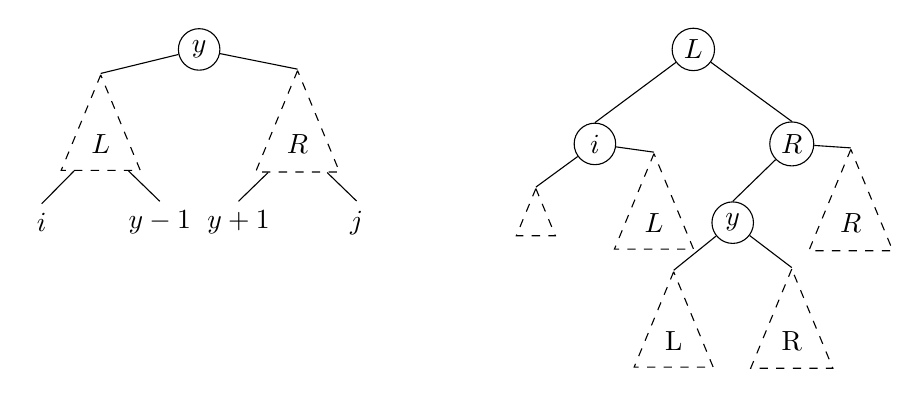
\begin{tikzpicture}
\node [tnode] (P) {$y$}
    [child anchor=north]
    child{
      node [subtree] {$L$}
      [child anchor=north]
      child{ node {$i$} }
      child{ node {$y-1$} }
    }
    child{
      node [subtree] {$R$}
      child{ node {$y+1$} }
      child{ node {$j$} }
    }
;
\node [tnode, right of=P, right=5cm] (T) {$L$}
    [child anchor=north]
    child{
      node [tnode] {$i$}
      [child anchor=north]
      child{ node [subtree] {\ } }
      child{ node [subtree] {$L$} }
    }
    child{
      node [tnode] {$R$}
      [child anchor=north]
      child{ node [tnode] {$y$}
        [child anchor=north]
        child{ node [subtree] {L} }
        child{ node [subtree] {R} }
      }
      child{ node [subtree] {$R$} }
    }
;
\end{tikzpicture}

Define $z(y)$ be the highest node in $T$ such that the path from the root passes through nodes both from $L$ and from $R$.

Let $LCA(a,b)$ be the lowest common ancestor of both $a$ and $b$.
The highest node from $L$ is $LCA(i, y)$. The highest node from $R$ is $LCA(y,j)$.

\paragraph{Claim}
One of $LCA(i,y)$ and $LCA(y,j)$ is an ancestor of the other.

\paragraph{Claim}
$z(y)$ is the lowest of $LCA(i,y)$ and $LCA(y,j)$.

\paragraph{Claim}
$z(y)\ne z(y')$ for any $y \ne y'$

\paragraph{Claim}
If $z(y)=LCA(y,j)$, then all the nodes in $R$ are descendants of $z(y)$. A similar claim for the converse is also made.

\paragraph{Claim}
$z(y)$ only changes when we touch $z(y)$ (when accessing or rotating $T$).

A visual proof of the second property was done on the whiteboard (using colors).

\section{Tango trees}
Binary search tree that for any sequence $\sigma$ does $W(P, \sigma) \log \log n$ operations, where $P$ is a balanced static tree.

The basic idea is to break up the tree into favored paths.

\paragraph{Example:}\ \\
%TODO: draw the favored paths in a different color
%TODO: draw groups around "favored" paths 0, 3-1-2, 4, 5-6, 7-11-13-14, 8-9, 10, 12.
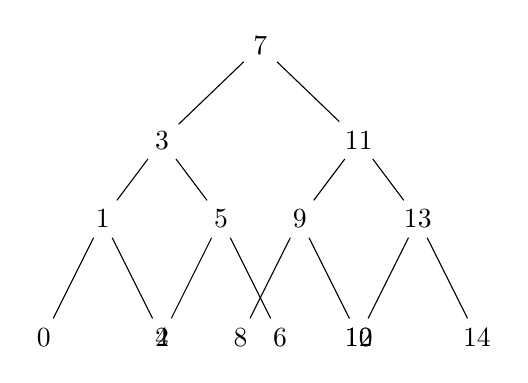
\begin{tikzpicture}
\node (P) {7}
  child{ node {3}
    child{ node {1}
      child{ node {0} }
      child{ node {2} }
    }
    child{ node {5}
      child{ node {4} }
      child{ node {6} }
    }
  }
  child{ node {11}
    child{ node {9}
      child{ node {8} }
      child{ node {10} }
    }
    child{ node {13}
      child{ node {12} }
      child{ node {14} }
    }
  }
;
\end{tikzpicture}

We will represent each "favored" path using a BST. Each BST has $O(\log n)$ nodes.
For each node $x$ in each BST, we keep a pointer to the root of the BST which contains the unfavored branch of $x$.
The depth of $x$ in $P$.
The maximum depth in $P$ of all the nodes underneath $x$ in the BST.

\paragraph{Example:}\ \\
\begin{tikzpicture}
\node [right of=P, right=4cm] (P1) {13}
  child{ node {11}
    child{ node {7} }
  }
  child{ node {14} }
;
\end{tikzpicture}

\paragraph{$\text{access}(x)$:}
Start from the BST that contains the root of $P$ (the favored path).
Search for predecessor and successor of $x$.
If we have not found $x$ in the BST, we continue to the unfavored path of either the predecessor or successor.
If we change the favored paths, we need to update the BSTs.

\subparagraph{Complexity}
Searching for the pred/succ: $O(\log\log n)$. Checking which tree $x$ belongs to costs us $O(1)$. Each time we switch BSTs to the unfavored branch, this costs OPT $O(1)$.

Therefore, for a sequence $\sigma$ of operations it costs us $O(W(P, \sigma) \cdot \lg\lg n)$.

\paragraph{Updating the favored path BSTs}
We want to cut the previously favored subtree, and link the new (using split/join). These cost us $O(\lg\lg n)$.
However, we need to split these by the maximum depth.
Mark l and r as the smallest and largest elements in the previously favored branch of $x$ in $P$.
Note that we can split based on some interval. Next week we will show the specifics of this operation.



\end{document}
